
En este capítulo se describirán los métodos usados para llevar a cabo las simulaciones.

Para realizar las simulaciones se utilizó el programa LAMMPS (Large-scale Atomic/Molecular Massively Parallel Simulator)~\cite{plimpton}.
Es un software de código libre distribuido bajo los términos de GPL.
LAMMPS se caracteriza por hacer uso de las listas de vecinos para efectuar cálculos que permiten reducir la 
complejidad algorítmica, permite correr las simulaciones en un único procesador o en paralelo (valiéndose de técnicas message-passing y descomposición espacial del dominio de simulación), además cuenta con una gran cantidad de funciones implementadas orientadas al uso de simulaciones de dinámica molecular. \\

Todas las simulaciones constaron de N individuos en un recinto cuadrado cuyo tamaño estaba ligado a la cantidad de
peatones de modo tal que mantenga constante la densidad. En una de las paredes se ubicaron una o dos puertas. Las puertas se ubicaban simétricamente respecto del medio para evitar efectos de borde. Cuando el recinto tenía dos salidas, ambas se fijaban del mismo ancho.
Las condiciones iniciales se detallan en la subsección \ref{ci}.  Luego del instante inicial, los agentes cambiaban su velocidad acorde a la velocidad de deseo (parámetro asociado al apuro) configurada de forma tal que los individuos evacúen por la puerta más cercana. Una vez que los individuos abandonaban el recinto no se los reinyectaba. De esta forma, al evacuar dejaban de importar sus observables. \\

La información era guardada cada 0,05~s. Para integrar las ecuaciones de movimiento se utilizó el algoritmo de Verlet. 

Los gráficos de la figura \ref{sim} representan el estado inicial de una simulación (izquierda) donde los individuos están ordenados en un arreglo periódico cuadrado. La imagen de la derecha muestra el estado 50000 iteraciones después (luego de 5 segundos de simulación). Puede verse que para ese entonces la multitud forma uan estructura de "semi círculo" en torno a la salida. Esta fenómeno emergente es propio de la dinámica granular~\cite{To} y característico de las evacuaciones en estado de pánico~\cite{Helbing1}  

\begin{figure}[H]
    \centering
    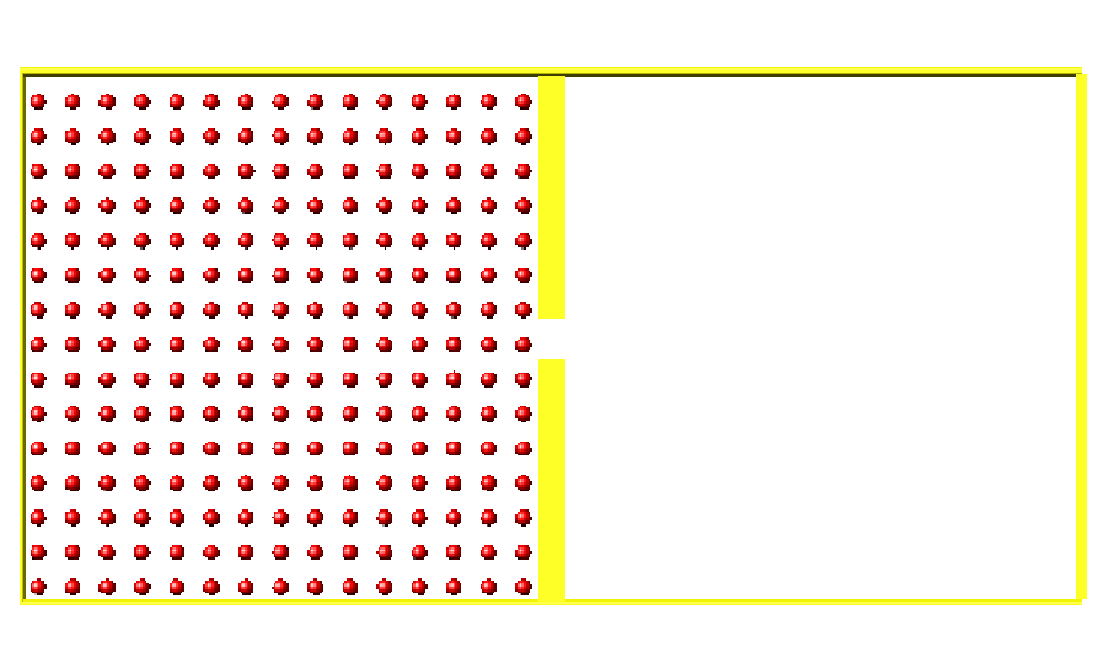
\includegraphics[scale=0.45]{figuras/0.eps}
    \hfill   
    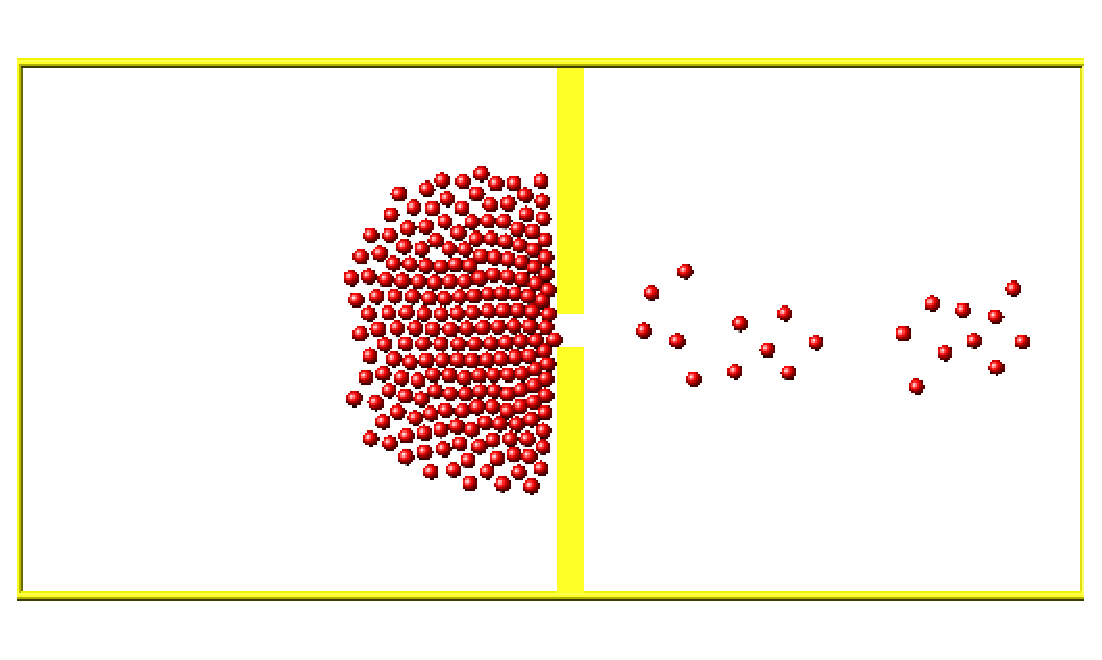
\includegraphics[scale=0.45]{figuras/500.eps}
     \caption[width=5cm]{Izquierda: Estado inicial de una simulación de 225 individuos en un recinto de 20$\times$20~m. Derecha: Estado de la simulación en la iteración 50000. }
    \label{sim}
\end{figure}

Con el fin de compatibilizar el modelo de fuerza social con LAMMPS, se crearon varios módulos con las fuerzas que caracterizan a este modelo. Todos estos fueron escritos en c++. En la  sección \ref{modulos} se describe cada uno de ellos. 
En la sección \ref{med realizadas} se detallarán los distintos tipos de mediciones llevadas a cabo.

\subsection{\label{ci}Condiciones iniciales}

Para todas los sistemas estudiados se configuró un arreglo bidimensional de individuos, ordenados inicialmente tipo red cuadrada, con una densidad de 0,6~personas/m$^2$, similar al límite de las regulaciones actuales~\cite{mysen} (con esta distancia la interacción de repulsión social es despreciable). Todos los individuos tenían una velocidad aleatoria con una distribución gausiana centrada en cero. El módulo de la velcidad inicial de los peatones se fijó con el comando {\tt velocity} de lammps. Esta instrucción requiere la "temperatura" del sistema. La misma se vincula con la energía cinética mediante la siguiente expresión

\begin{equation}
v=\sqrt{\frac{2k_b}{m}T}
\end{equation}

donde $k_b$ es la constante de Boltzman y T es la temperarura configurada en la simulación
El valor usado de temperatura fue $10^{23}$ de modo que el módulo de la velocidad inicial sea $v=1.19$~m/s




\section{\label{modulos}Módulos}

{\Large {\tt pair\_social}}

Este módulo se hizo para incluir la fuerza de repulsión social ($\mathbf{f}_s^{(ij)}$) del modelo de Helbing (ver sección \ref{sfm}). Toma como parámetros la constante B y la distancia de corte (si los individuos están separados por una distancia mayor a este corte, la fuerza social entre ellos no se calcula).
Otros parámetros son agregados a través de la función pair\_coef. Estos son la constante A del modelo de Helbing, la distancia 
de corte y el radio de los individuos. Los valores utilizados fueron: A $=$ 2000, B$=$ 0,08 r\_cut $=$3,5 d$=$ 0,30.
La elección de la distancia de corte se tomó de modo tal que la fuerza social que sienten individuos separados a esa distancia
sea despreciable ($\sim$ 10$^{-12}$ N). El resto de los parámetros fueron extraídos de la bibliografía del modelo de fuerza social~\cite{Helbing1}.

{\Large {\tt pair\_gran\_social}}

Se creó para que exista rozamiento entre los individuos que están en contacto. Requiere como parámetro el valor de la constante de rozamiento, el mismo fue $\kappa =2,4 \times 10^5$~kgm$^{-1}$s$^{-1}$. Tanto el valor de $\kappa$ como la expresión de la fuerza concuerdan con los del modelo de Helbing.

{\Large {\tt fix\_wall\_social} y {\tt fix\_wall\_gran}}

Estos módulos son análogos a pair\_social y pair\_gran\_social pero aplicados a las fuerzas de interacción entre los individuos y las paredes. El primero simula la fuerza de repulsión y posee los mismos parámetros que la repulsión entre individuos mientras que el segundo modela la fuerza de rozamiento dinámico. 

{\Large {\tt fix\_social\_self} y {\tt fix\_social\_self\_multi}}

La fuerza de deseo del modelo de Helbing fue simulada con estos módulos. El primero se usó para los recintos con una única puerta mientras que el segundo para recintos con dos. 
fix\_social\_self requiere como parámetro la masa de los individuos y la velocidad de deseo. El target que tiene cada individuo, depende de la posición en donde se encuentre. Por cada puerta hay tres targets: superior, medio e inferior. El medio está ubicado en la mitad de la puerta, los otros 0,3 m por encima y por debajo.  Los individuos cuya posición en la coordenada 'y' sea mayor (menor) que el target superior (inferior) actualizan su velocidad para apuntar al target superior (inferior). Si se encuentran en medio de éstos, apuntan al centro de la puerta. De este modo los peatones siempre se dirigen al target más cercano.\\  

Cuando se simularon recintos con dos puertas se usó fix$\_$social$\_$self$\_$multi, sus parámetros son: la masa de los individuos, la velocidad de deseo y el gap (la distancia de separación entre puertas). Si el gap es nulo, las dos puertas están unidas (formando una única puerta ancha). En este caso, se establecen tres targets: el superior (inferior), que está 0.3 m debajo (encima) del final de la puerta superior (inferior). Los individuos que se encuentran en el medio apuntan al centro (al igual que en el caso de una única puerta).
Si el gap no es nulo, es decir, existe una porción de pared entre ambas puertas, la dirección de la velocidad de los individuos se actualiza de forma análoga al caso de una puerta. De esta forma los individuos siempre buscan la salida más cercana. 

{\Large {\tt compute\_social\_pressure}}

Calcula la función de presión social de la expresión (\eqref{pv}) despreciando el término cinético y el factor 1/2. Para cada timestep devuelve un vector con la presión que soporta cada peatón como consecuencia de la interacción con sus vecinos. 

{\Large \tt {compute\_dijkstra\_atom}}

Rotula con la misma etiqueta a todos los elementos que forman parte de un blocking cluster. Requiere como parámetro las posiciones en la coordenada 'y' de los puntos de origen y terminación del blocking cluster y la posición de la pared en la coordenada 'x'. Para cada timestep devuelve un vector con N componentes (siendo N la cantidad de peatones). Cada una de estas componentes esta asociada a un individuo; toma un número distinto de cero cuando el individuo forma parte de un cluster de bloqueo y cero en caso contrario.

\section{\label{Muestras de performace} Muestras de performance} 

Se llevaron a cabo dos simulaciones (partículas centradas y partículas en hilera) para poner a prueba el módulo que calcula la presión y su relación con la ecuación del virial. \\ 

\subsection{Partículas centradas}

Se simuló un conjunto de 19 partículas cuyo target es el origen de coordenadas. Con una velocidad de deseo $v_d=4$~m/s en módulo. En el estado estacionario la disposición de las partículas es tal como se muestra en la figura \ref{central} . Las partículas se encuentran casi estáticas; poseen una pequeña oscilación en torno a la posición de equilibrio. 

\begin{figure}[H]
    \centering
        \includegraphics[scale=0.5]{figuras/central.png}
    \caption[width=5cm]{Esquema de las partículas. Partícula central rodeada por 6 primeros vecinos y doce segundos vecinos.}
    \label{central}
\end{figure}


El resultado de esta simulación es el conjunto de valores que se exhiben en las tablas de abajo. Éstos son la distancia al origen y la presión social que siente cada individuo. 

%\begin{table}[H]
\begin{center}
%\caption{Resultados numéricos de la simulación.}
\label{my-label}
\begin{tabular}{|l|l|}
\hline
Distancia (m) & Presión (N.m) \\ \hline
1,48          & 664,0       \\ \hline
1,26          & 999,9       \\ \hline
1,49          & 653,3       \\ \hline
1,48          & 664,0       \\ \hline
1,27          & 988,7       \\ \hline
0,7           & 1820,5       \\ \hline
0,7           & 1820,9       \\ \hline
0,0           & 2340,2       \\ \hline
0,7           & 1829,9       \\ \hline
0,7           & 1833,5       \\ \hline
\end{tabular}
\quad
\begin{tabular}{|l|l|}
\hline
Distancia (m) & Presión (N.m) \\ \hline
1,26          & 989,8       \\ \hline
1,49          & 655,2       \\ \hline
1,26          & 991,9       \\ \hline
1,49          & 653,7        \\ \hline
0,7           & 1828,0       \\ \hline
1,26          & 1004,1       \\ \hline
0,7           & 1833,6       \\ \hline
1,48          & 663,1       \\ \hline
1,26          & 1002,1       \\ \hline
\end{tabular}
%\end{table}
\end{center}


Sumar todos los valores de presión social y dividir por dos da como resultado el lado izquierdo de la ecuación (\ref{virial2}).
\begin{equation}
 \displaystyle\sum_{i=1}^N\langle3P_iV_i\rangle = 11618.6\ \text{N.m}
\end{equation}

La suma de todas las distancias multiplicada por la fuerza de deseo $f_d=mv_d/\tau$ da como resultado el lado derecho (despreciando el primer término porque no hay interacción con paredes):

\begin{equation}
 -3\mathcal{PV} -\displaystyle\sum_{i=1}^N \langle
\mathbf{r}_i\cdot\mathbf{f}_d^{(i)}\rangle\ =  11580.8\ \text{N.m}
\end{equation}

Ambos valores son cercanos. Por lo tanto, el resultado de esta simulación verifica la relación del virial (\ref{virial2}).


\subsection{Partículas en hilera}

Se creó un código que mide la presión que soportan los individuos dispuestos en hilera como muestra la figura \ref{hilera} 

\begin{figure}[!htbp]
\center
\includegraphics[scale=1]{figuras/hilera.eps}
\caption{\label{hilera}}
% done with figuras_presion.odg
\end{figure}

Los resultados se muestran en la tabla \ref{simulados}. La misma está ordenada del individuo más cercano al más lejano de la pared. La presión disminuye conforme se alejan de la pared y el valor de presión aumenta con la cantidad de individuos.\\
En la tabla \ref{teoricos} se muestran valores de presión teóricos (calculados a partir de las fórmulas \ref{eqn_7}, \ref{eqn_8} y \ref{eqn_9} del apéndice \ref{appendix:presion}). Las magnitudes de presión son comparables a las simuladas y el comportamiento a grandes rasgos es similar (las partículas más presionadas son las que se encuentran más cerca de la pared y aumentar N aumenta la presión general)  

\begin{table}[h!]
\caption {Valores simulados de $6P_iV_i$ para $v_d=4\,$m/s.}
\label{simulados}
\begin{center}
\begin{tabular}{|l|cccccc|}
\hline
      & \multicolumn{6}{c|}{$N$} \\
\hline
$i$   &  1   &   2    &  3       &  4     &  5     &   6     \\
\hline
 1    &  --- &  ---   &  ---     & ---    & ---    & ---     \\
 2    &      &  393.2 &  1116.7  & 1751.4 & 2362.2 & 2927.0  \\
 3    &      &        &  393.03  & 1113.8 & 1761.7 & 2355.1  \\
 4    &      &        &          & 391.45 & 1120.3 & 1755.4  \\
 5    &      &        &          &        & 394.03 & 1117.0  \\
 6    &      &        &          &        &        & 393.03  \\
\hline
\end{tabular}
\end{center}
\end{table}



\begin{table}[h!]
\caption {Valores teóricos de $6P_iV_i$ para $v_d=4\,$m/s.}
\label{teoricos}
\begin{center}
\begin{tabular}{|l|cccccc|}
\hline
      & \multicolumn{6}{c|}{$N$} \\
\hline
$i$   &  1         &   2        &  3       &  4     &  5     &   6   \\
\hline
 1    &  225.03    &  780.98    &  1251.4  & 1683.1 & 2088.3 & 2473.2 \\
 2    &            &  393.03    &  1117.0  & 1755.4 & 2355.1 & 2928.3 \\
 3    &            &            &  393.03  & 1117.0 & 1755.4 & 2355.1 \\
 4    &            &            &          & 393.03 & 1117.0 & 1755.4 \\
 5    &            &            &          &        & 393.03 & 1117.0 \\
 6    &            &            &          &        &        & 393.03 \\
\hline
\end{tabular}
\end{center}
\end{table}


En esta sección se verificó que los resultados simulados verifican la relación del virial (partículas centradas) y a su vez concuerdan con los cálculos teóricos (partículas en hilera)


\section{\label{med realizadas} Mediciones Realizadas}

{\Large Isobaras}

Se hicieron simulaciones con el módulo que cuantifica la presión social sobre cada agente. De esta
forma se obtuvieron datos de presión y posición en función del tiempo para cada individuo. Con Python se creó una grilla con celdas de 1~m$^2$. Se sumó la presión asociada a cada una y se la normalizó por la cantidad de individuos que pasaron por dicha celda. Así se obtuvo la presión promedio en cada región del recinto. Luego se generó un gráfico de isobaras (contour map). Los datos de cada celda fueron promediados con los de sus celdas vecinas para obtener gráficos de presiones "suavizados".

%Se hicieron simulaciones con el módulo que cuantifica la presión social sobre cada agente. De esta forma se obtuvieron datos de presión y ubicación en función del tiempo para cada individuo. Éstos fueron analizados con Python para generar gráficos de isobaras (contour maps). Se creó una grilla con celdas de 1~m$^2$. Se sumó la presión asociada a cada una y se la normalizó por la cantidad de individuos que pasaron por dicha celda. Así se obtuvo la presión promedio en cada región del recinto.   

Estos mapas de presión se hicieron para recintos de 20$\times$20~m con 225 individuos. La habitaión contaba con una única puerta de ancho: 1,2~m, 2,4~m, 3,6~m o con dos puertas de 1.2~m separadas a distintas distancias. Para cada tipo de medición se efectuaron 30 simulaciones. Cada una de estas se terminó al evacuar 100 individuos. 

{\Large Flujo de velocidad}

De forma análoga se medió la velocidad de cada individuo ($v_x$ y $v_y$) con el fin de realizar gráficos de líneas de corriente (stream plots). Las condiciones de medición y los recintos de simulación fueron los mismos que los del gráfico de isobaras. 

{\Large Presión y velocidad en función del tiempo}

Para un peatón cuya posición inicial es (x,y)=(12.35,8.45) en un recinto de 20$\times$20~m con 225 individuos se midió la presión social y velocidad (módulo) en función del tiempo desde que comienza la simulación hasta que logra evacuar. Estas simulaciones se hicieron para recintos con una única puerta de 1,2~m y 3,6~m. 

{\Large Tiempo de evacuación}

Se registró el tiempo que demora evacuar más del 70\% de los individuos en distintos recintos y bajo diferentes condiciones. Se hicieron mediciones en recintos de 20$\times$20~m, 30$\times$30~m y 40$\times$40~m con 225, 583 y 961 individuos respectivamente para diferentes velocidades de deseo (de 2~m/s a 8~m/s). Algunas mediciones se hicieron para estudiar la variación del tiempo de evacuación en función del gap y otras para confirmar el efecto "Faster is slower". 

{\Large Probabilidad de formar blocking clusters}

Mediante el módulo que identifica los individuos que conforman un blocking cluster se calculó el cociente entre el tiempo que la salida está bloqueada y el tiempo total de la evacuación. Este cociente es la probabilidad de formar blocking clusters. Se graficó esta probabilidad para clusters grandes y pequeños en recintos de 20$\times$20~m con 225 individuos con velocidad de deseo de 4~m/s, 6~m/s y recintos de 40$\times$40~m con 961 individuos con $v_d$=4~m/s. 30 iteraciones fueron realizadas para promediar los resultados. 

{\Large Presión en función de distancia a la puerta}

Se midió la presión (social) media en función de la distancia a la salida en recintos de 20$\times$20~m con 225 individuos. El ancho de la puerta fue 1,2~m. La velocidad de deseo 4~m/s. Se promedió el resultado de 30 iteraciones las cuales terminaban cuando 100 peatones abandonaban el recinto. Se llevaron a cabo dos tipos de análisis: en uno la distancia a la puerta fue dividida en intervalos de 0,3~m y en el otro fue dividida con celdas 1~m pero restringidas a 9,5~m $\le$ y $\le$ 10,5~m. \\

En el apéndice \ref{appendix:script} se presenta un script básico de Lammps con una descripción detallada del mismo. 


%%%%%%%%%%%%%%%%%%%%% Ver si queda o se va %%%%%%%%%%%%%%%%%%%
%A lo largo del trabajo se realizaron diversas simulaciones que permitieron caracterizar el comportamiento de multitudes evacuando en estado de pánico. En esta sección se mencionarán las simulaciones y técnicas de medición que se llevaron a cabo.\\

%Para estudiar el tiempo de evacuación en función de la distancia entre puertas se generó un código con un loop sobre la distancia de separación (gap). Para cada gap se realizaron 30 simulaciones con diferentes distribuciones de velocidad inicial para los individuos del recinto. Se midió sobre tres tipos de recintos, con 225, 580 y 961 individuos, siendo el tamaño de las habitaciones 20 $\times$ 20, 30 $\times$ 30 y 40 $\times$ 40 respectivamente. La densidad de individuos fue la misma en todos los casos (1.3 personas por cada metro longitudinal). Cada simulación se terminó cuando la cantidad de evacuados llegó a 160, 529 y 864 (según el tamaño del recinto); se registró el tiempo de evacuación en cada una . Con las 30 simulaciones por gap se calculó el promedio y desvio estándar, de esta forma pudo graficarse el tiempo de evacuación en función del gap. Para todas estas simulaciones, la velocidad de deseo se fijó en $v_d=4$~m/s excepto para el recinto con 225 individuos donde también se hicieron mediciones con $v_d=8$~m/s.  \\

